%% ----------------------------------------------------------------------------
% BIWI SA/MA thesis template
%
% Created 09/29/2006 by Andreas Ess
% Extended 13/02/2009 by Jan Lesniak - jlesniak@vision.ee.ethz.ch
%% ----------------------------------------------------------------------------
\newpage
\chapter{Qualitative Analysis}

\section{Selection}

\begin{figure}
\centering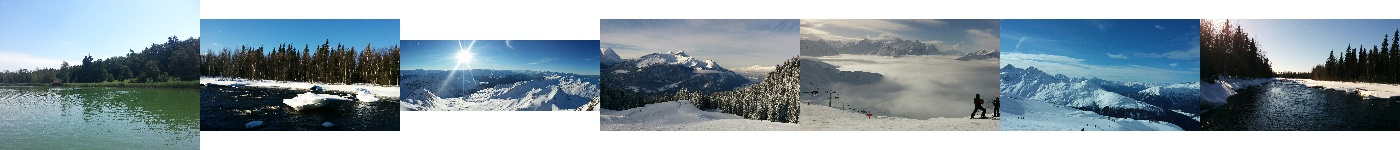
\includegraphics[width=1.0\columnwidth]{../figures/top7_suitable.jpg}
\caption{Top 7 suitable images in descending score order (Michael dataset)\label{fig:selection_top7}}
\end{figure}

Figure \ref{fig:selection_out1} shows 21 sample images from the Michael dataset.
These images, as mentioned before, can include undesirable objects such as text,
street signs, or store items.
As mentioned in section \ref{sec:method_cropping}, a SVM is trained using
features representing object classes.
When classifying the given images using this SVM, the resulting selection of
wallpaper candidates are shown in figure \ref{fig:selection_out2}.

\begin{figure}
\centering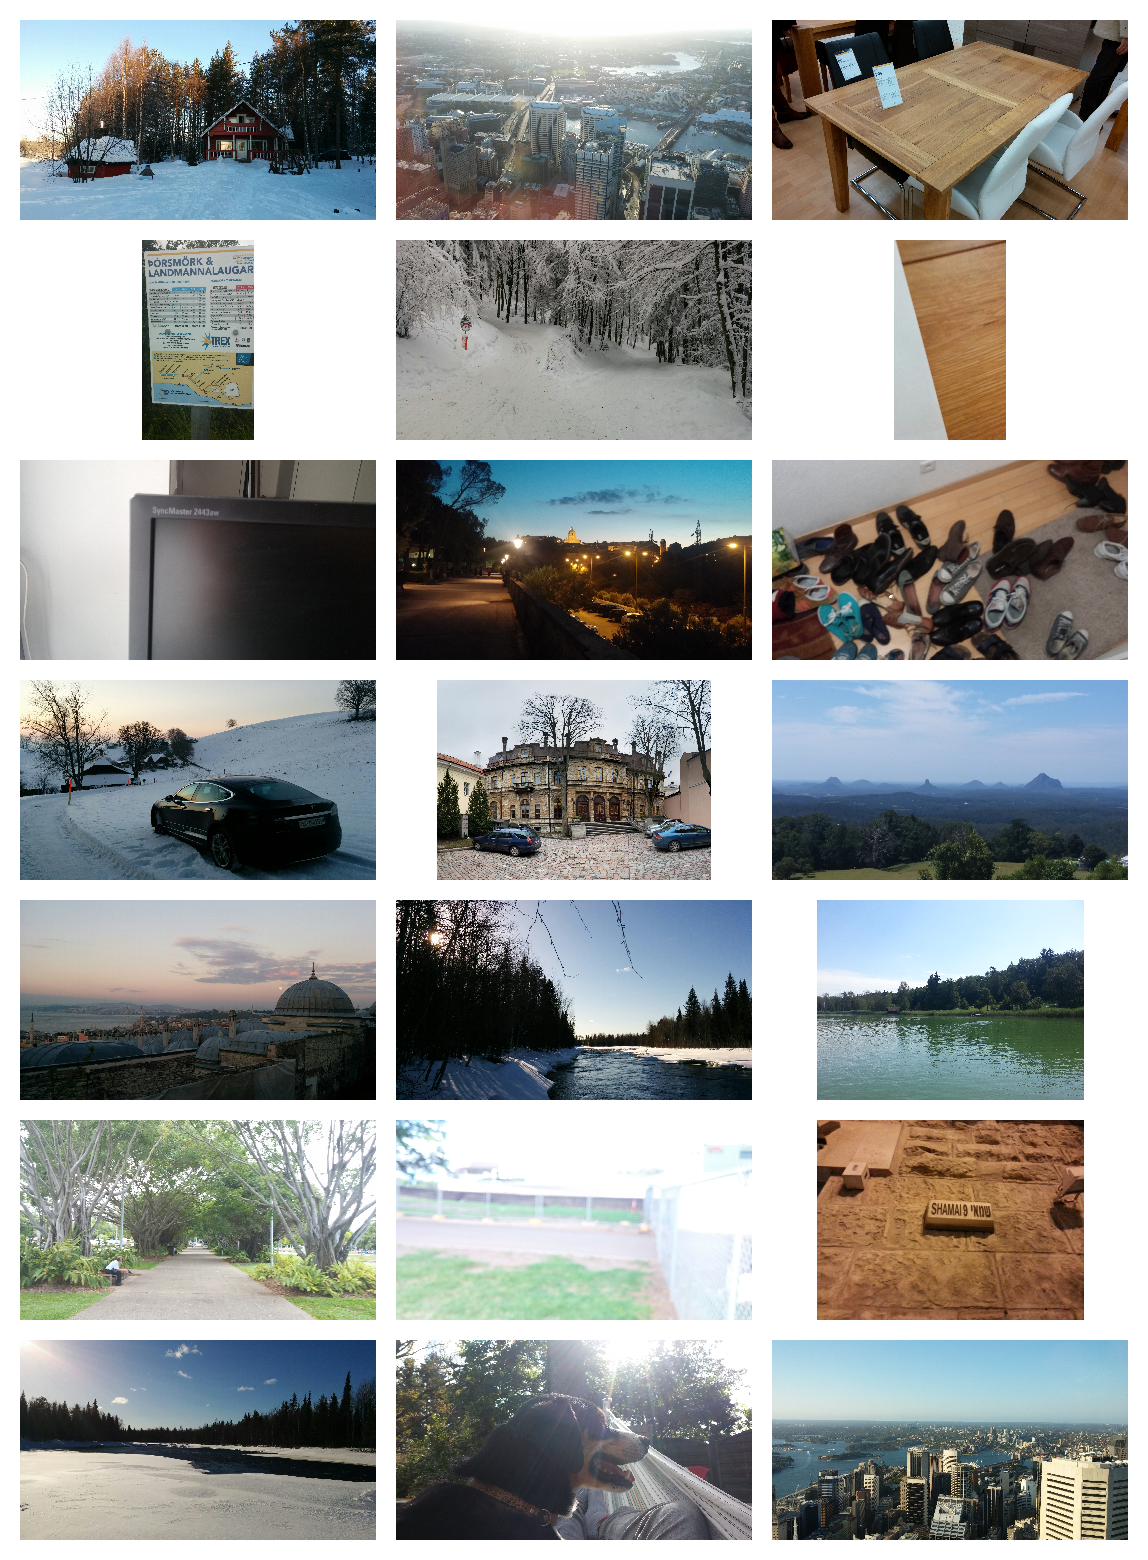
\includegraphics[width=0.9\columnwidth]{../figures/grid7x3_out1.png}
\caption{21 sample images from Michael dataset.\label{fig:selection_out1}}
\end{figure}

It can be seen qualitatively that images with undesirable objects have been
discarded, such as the image of furniture, a poster, or the model number
of electronic equipment.
Though in general photos with obviously undesirable objects are discarded as
appropriate, photos of city skylines or prominent single foreground objects for
example are not usually classified as being appropriate.
This is due to disagreements between annotators.
A larger number of annotations per image may help in this case.

\begin{figure}
\centering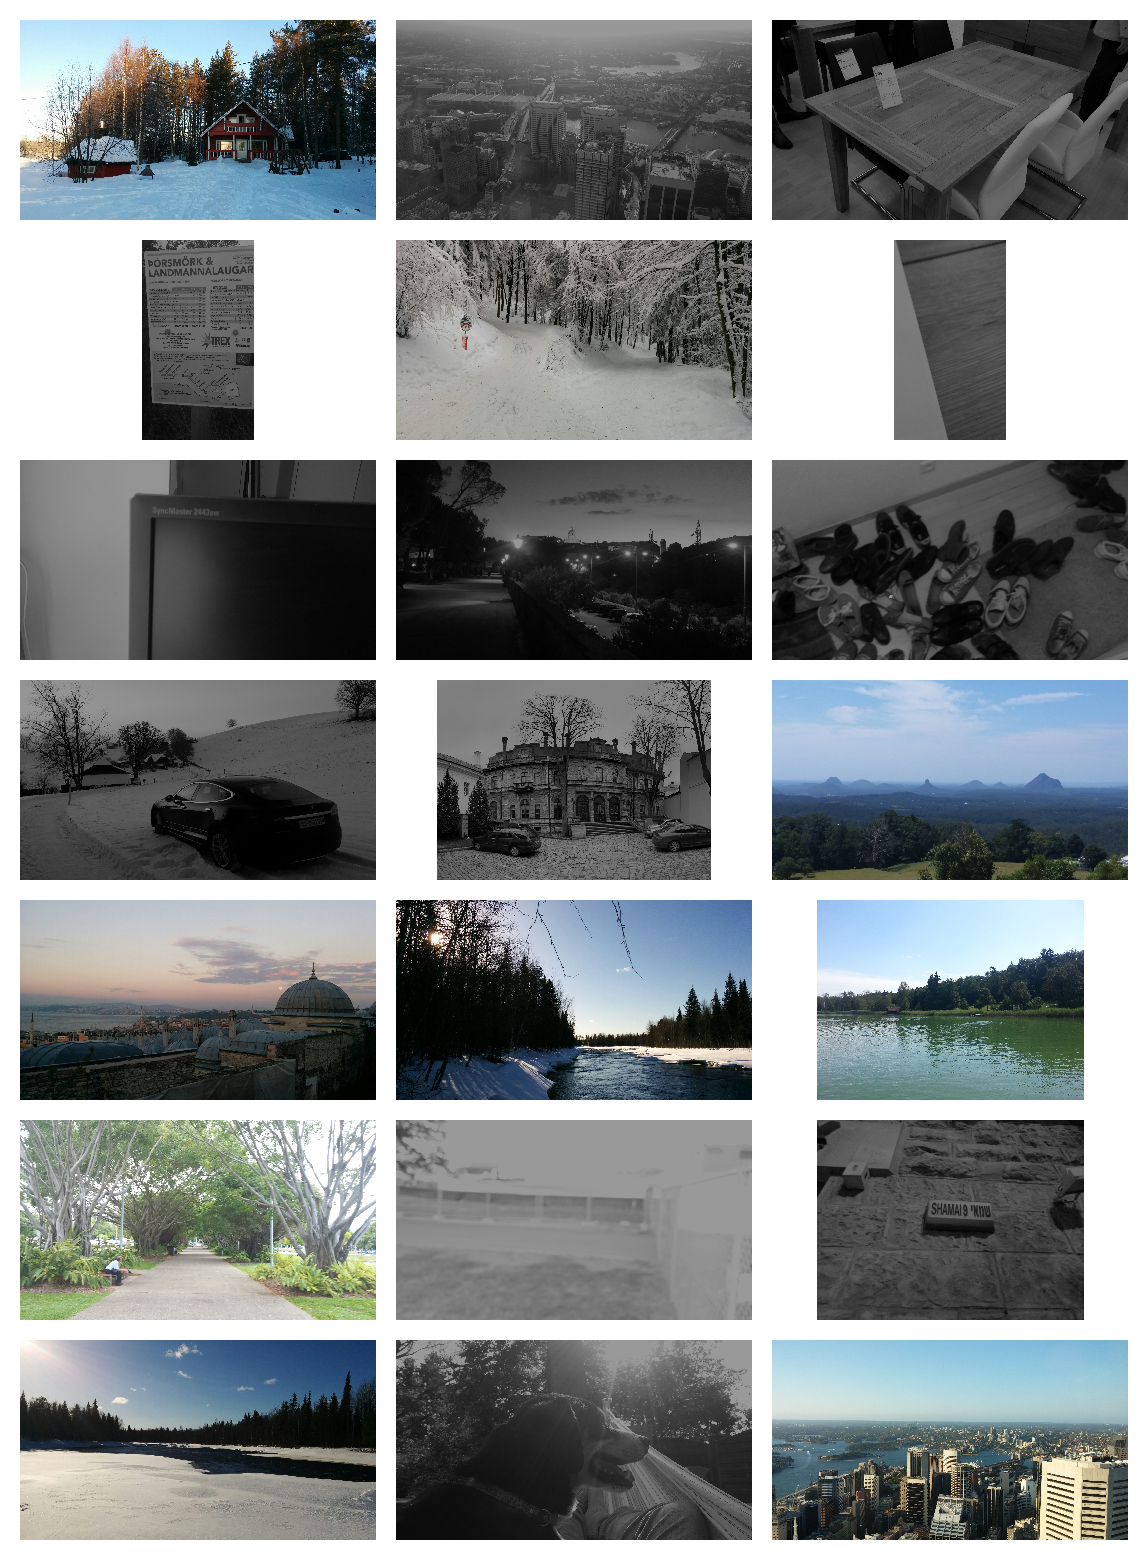
\includegraphics[width=0.9\columnwidth]{../figures/grid7x3_out2.png}
\caption{21 sample images from Michael dataset with images not selected dimmed
	and in grayscale.\label{fig:selection_out2}}
\end{figure}

When evaluating scores for all images in the Michael dataset, it can be seen in
figure \ref{fig:selection_top7} that images of distant natural landscapes attain
high scores.
Unlike scenes such as dark indoors and cityscapes, natural landscapes tend to be
classified as suitable by more annotators.

It should be noted that a single user's preference could be greatly different
from most other users where the purpose and intent of having a photo wallpaper
may differ.
For example, user A may desire to have dark and slightly artistic photos mainly
biasing towards indoor club scenes and long exposure shots at night.
User B might be a big fan of album art or concert photos, desiring objects or
scenes that we tend to assume to be undesirable.
It was actually the case in this study that using greatly conflicting
annotations caused issues in classification, where an annotator heavily favoured
dark scenes with low detail or discernible objects.

Further work could be done to perform a weighted average of multiple classifiers
depending on wallpaper preferences.

\newpage
\section{Cropping\label{sec:qualitative_cropping}}

The automatic cropping algorithm works quite well in general.
In the following figures, four images are shown per input image: the original
image, a saliency map, a gradient map, and the final cropped image.
It should be noted that brigher regions in a saliency map represent more
visually distinct regions, and brighter regions in a gradient map represent
regions with large changes in colour.

It is hoped that the saliency map emphasizes prominent objects well enough for
irrelevant or less important details to be left out of the final crop, and the
gradient map exhibit low values for background regions.
For the cases where this is true, it can be seen that the algorithm works very
well.

In figure \ref{fig:cropped_refocus} in particular, it can be seen that the most
prominent object is retargeted well.
This tends to result in better composed final images.
Some of the crops even exhibit some considerations of boundary simplicity.
Figure \ref{fig:cropped_simplicity} shows this effect better.
The classifier favours having lower gradient values on crop borders, leading to
crops which do not tend to intersect objects.
It should be noted that since the input gradient map is intentionally not
normalised, weaker boundaries can be included in crop boundaries.
As opposed to \cite{fang2014automatic}, the weighting of boundary simplicity is
not done using a fixed variable but by relying on the training of the SVM.

\begin{figure}
\centering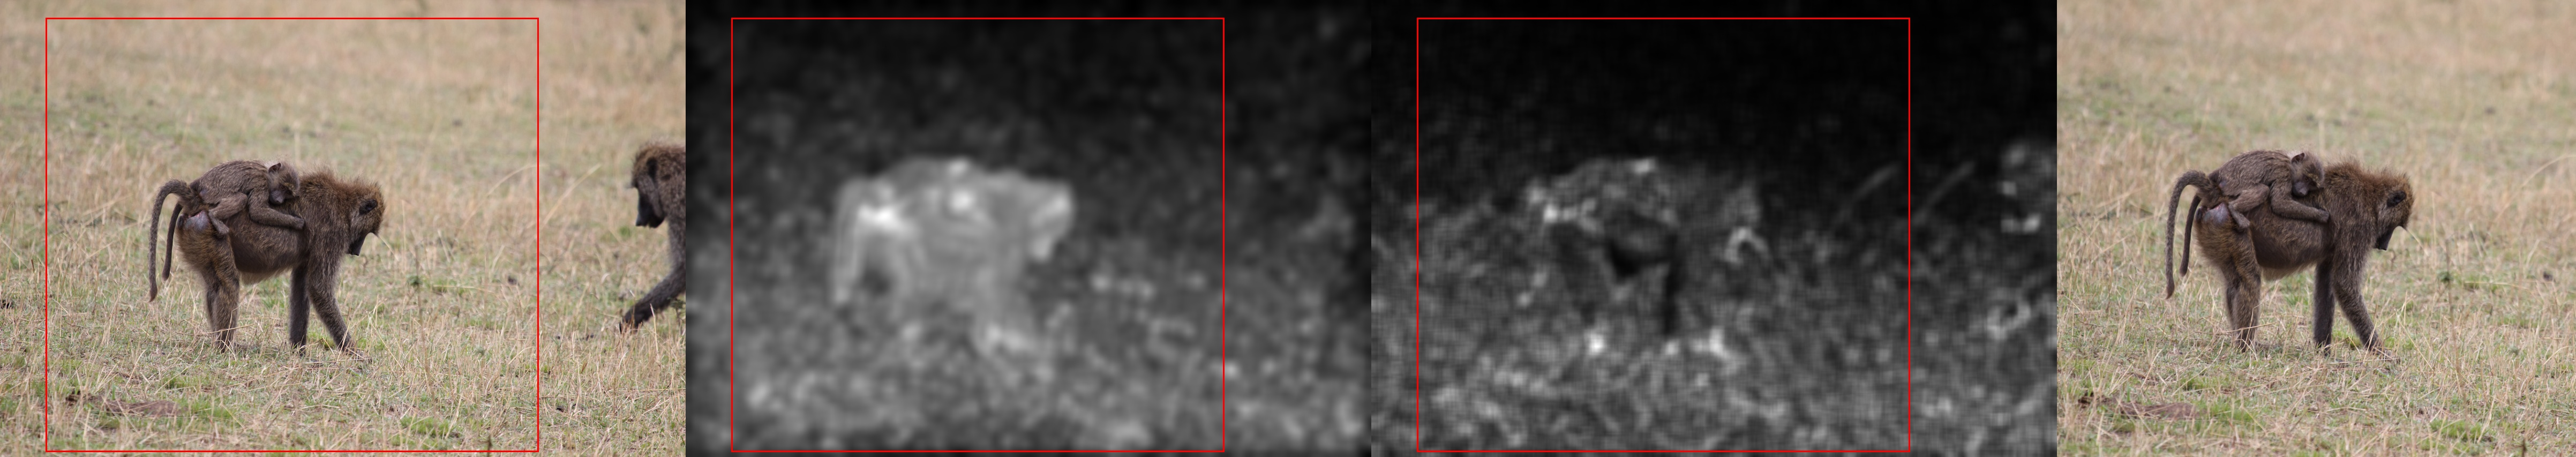
\includegraphics[width=0.9\columnwidth]{../figures/Chen_crops/isolate/IMG_0350.jpg}
\vskip3pt
\centering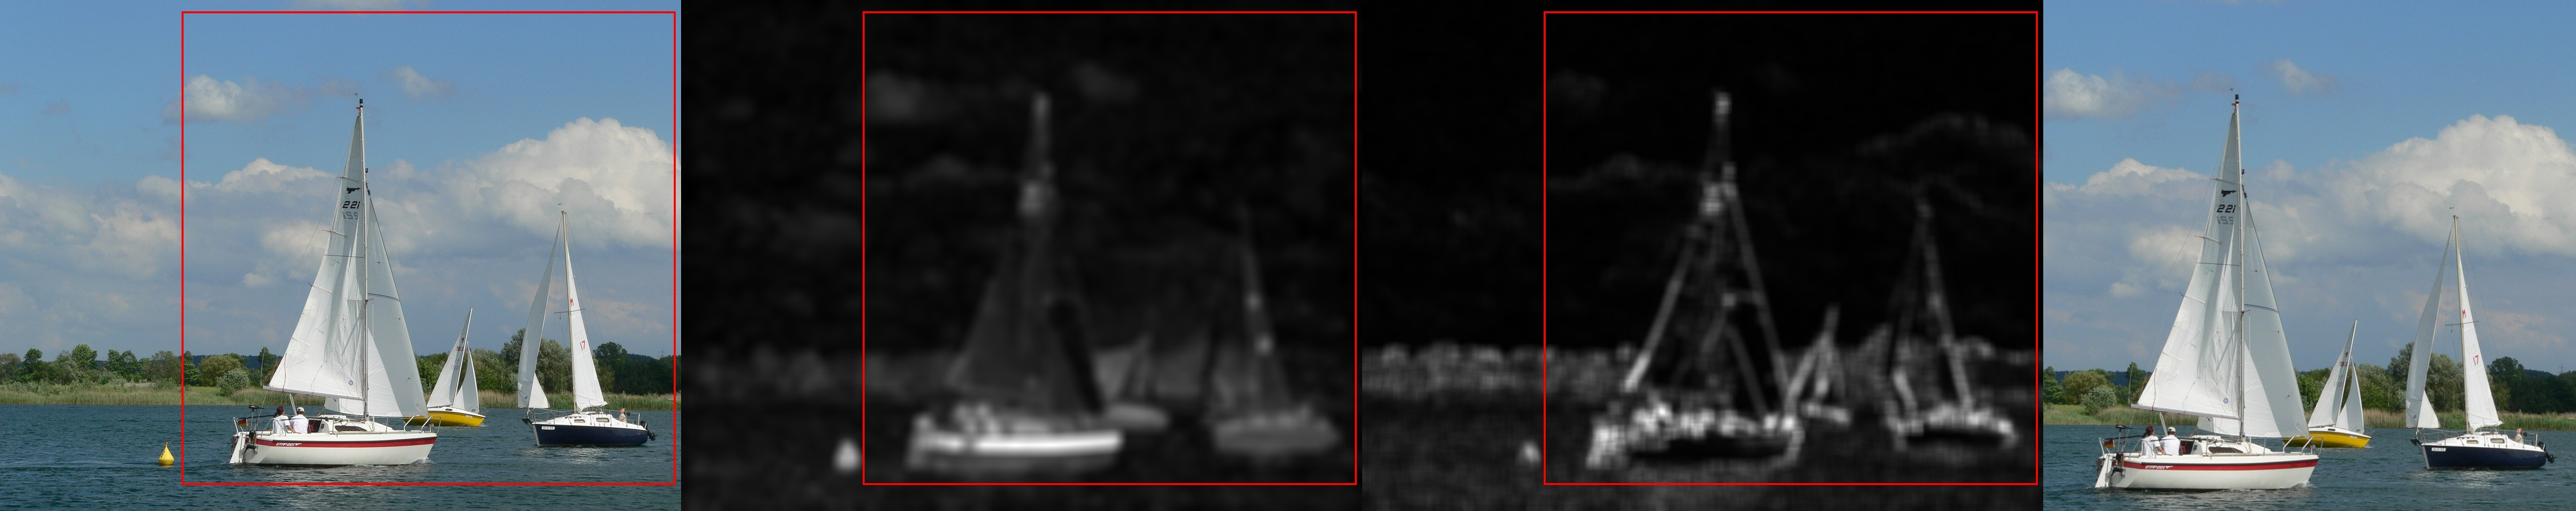
\includegraphics[width=0.9\columnwidth]{../figures/Chen_crops/refocus/146931510_Large.jpg}
\vskip3pt
\centering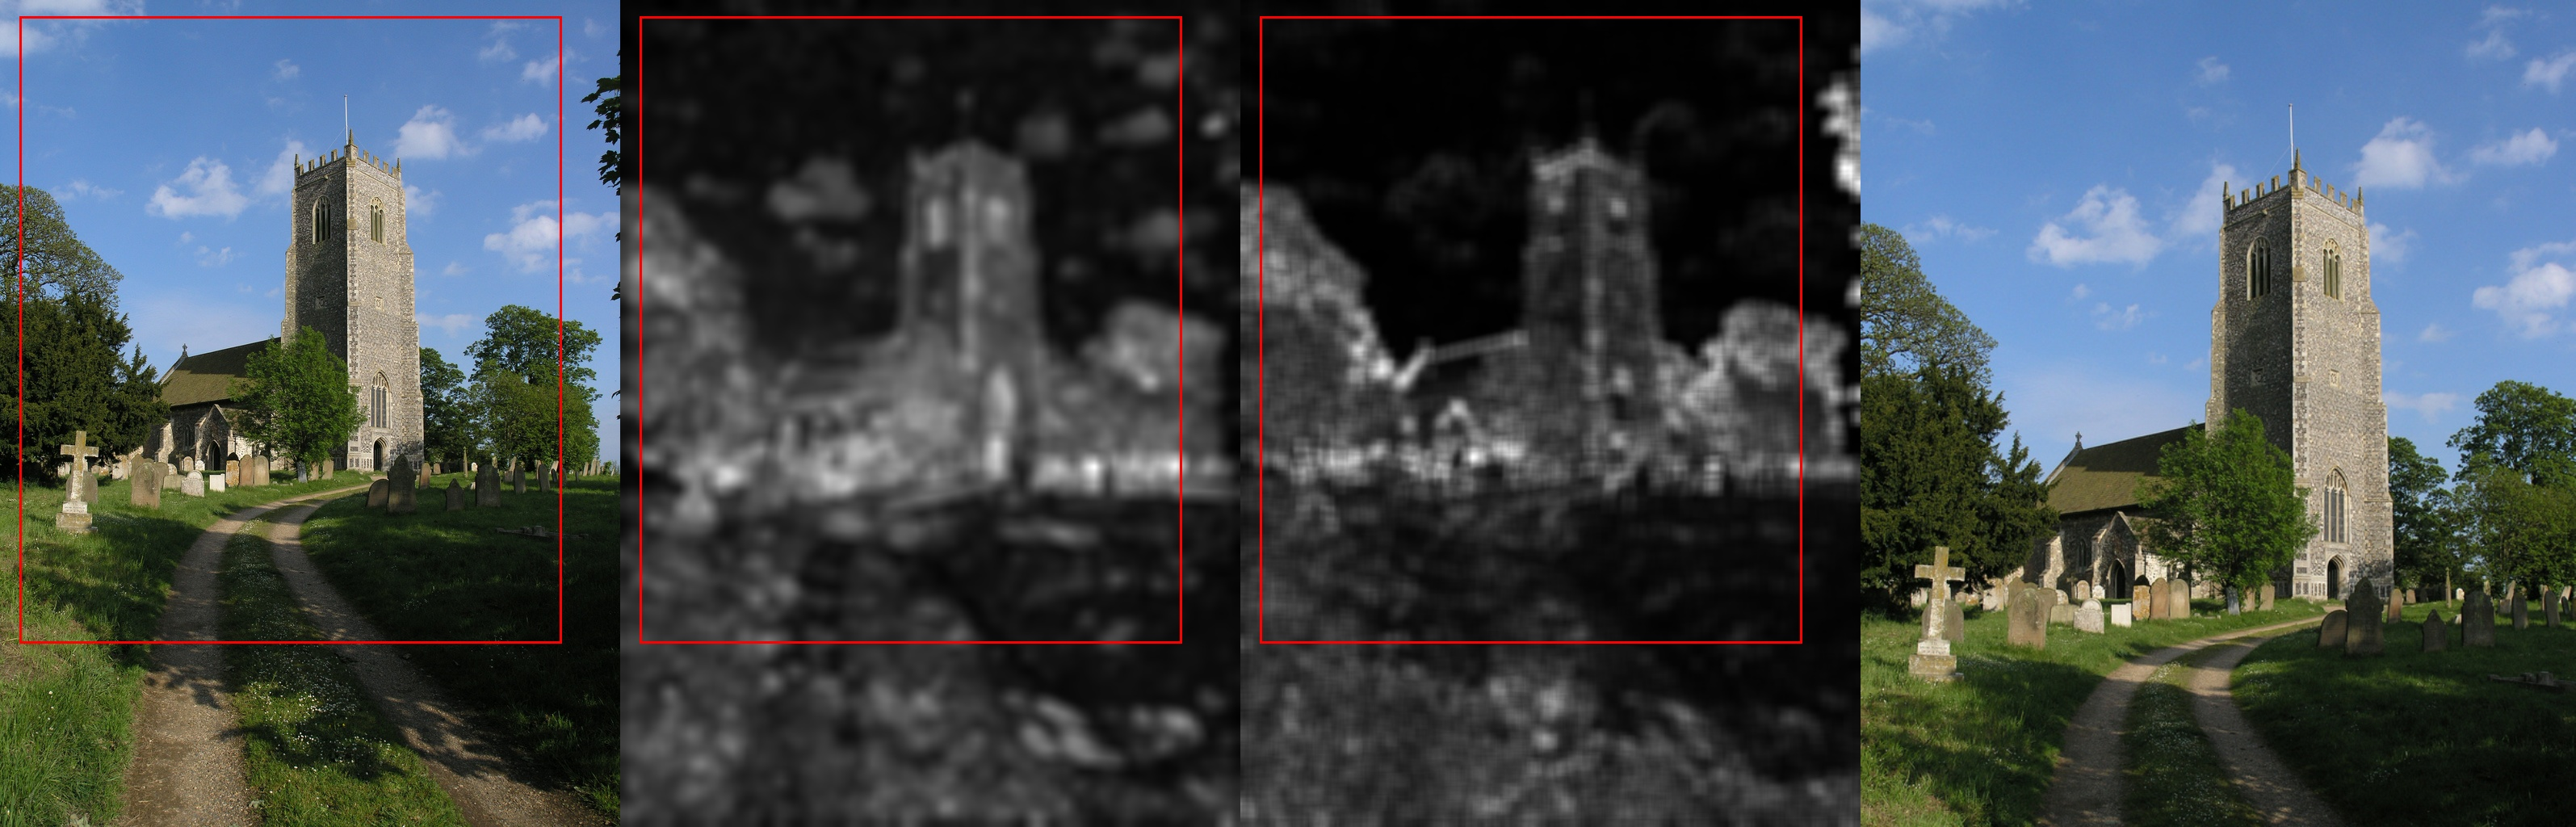
\includegraphics[width=0.9\columnwidth]{../figures/Chen_crops/refocus/1845766133_Large.jpg}
\vskip3pt
\centering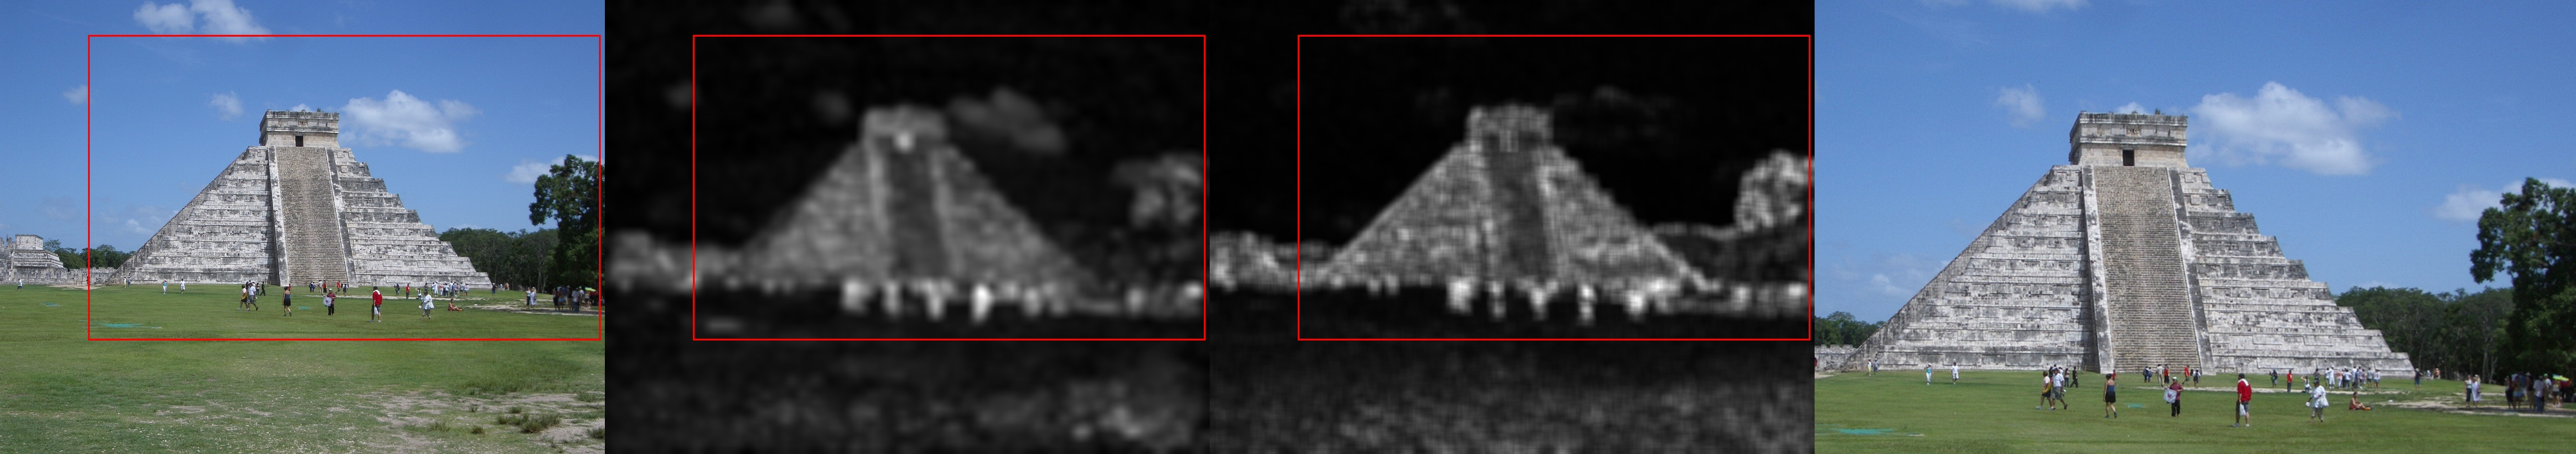
\includegraphics[width=0.9\columnwidth]{../figures/Chen_crops/refocus/236441280_Large.jpg}
\vskip3pt
\centering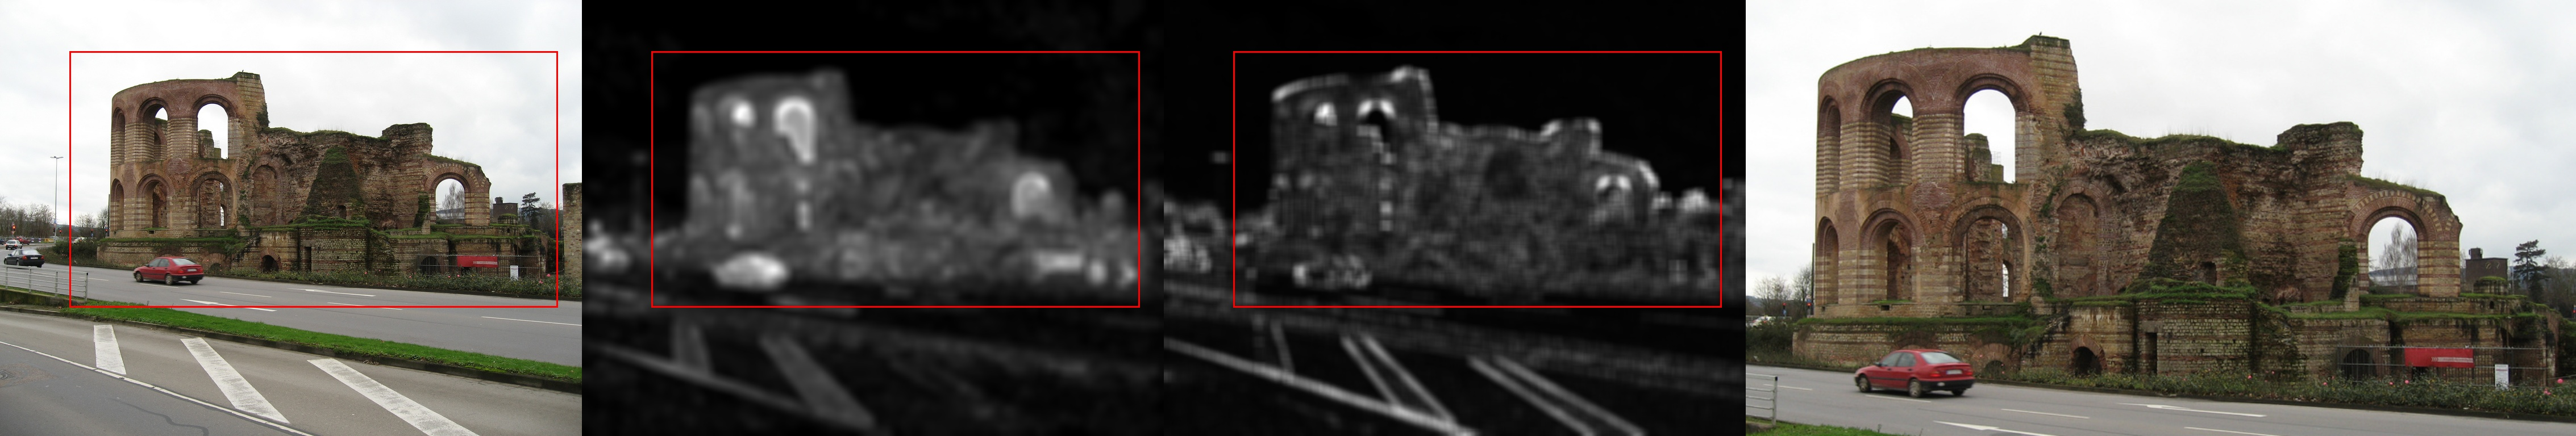
\includegraphics[width=0.9\columnwidth]{../figures/Chen_crops/refocus/406813066_Large.jpg}
\vskip3pt
\centering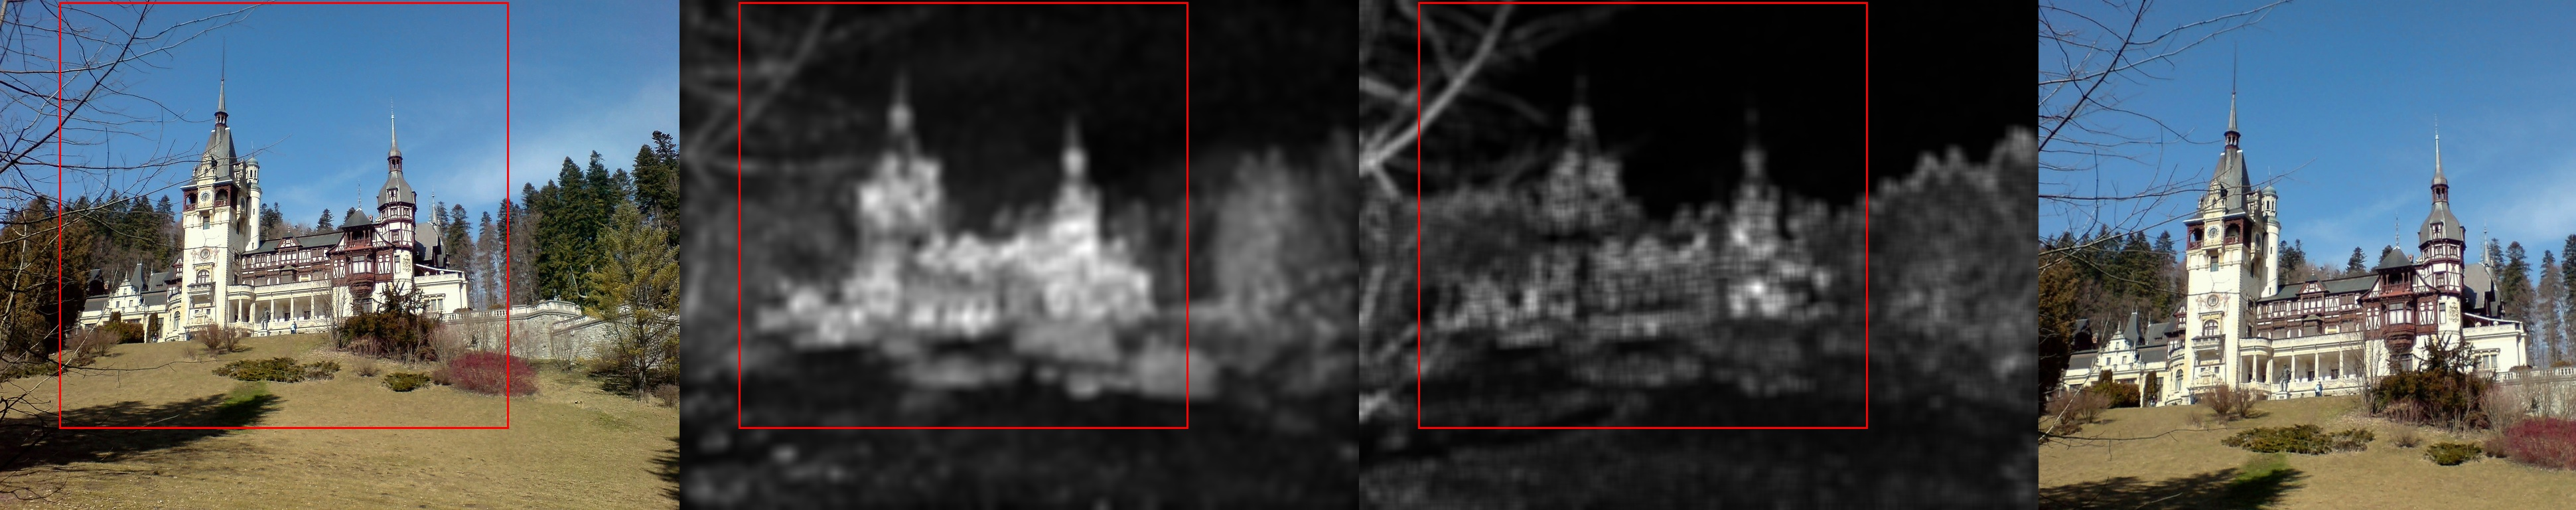
\includegraphics[width=0.9\columnwidth]{../figures/Chen_crops/refocus/420319741_Large.jpg}
\vskip3pt
\small{(From left to right: original image, saliency map, gradient map, final cropped image)}
\caption{Crops with main objects isolated and centered.\label{fig:cropped_refocus}}
\end{figure}

\begin{figure}
\centering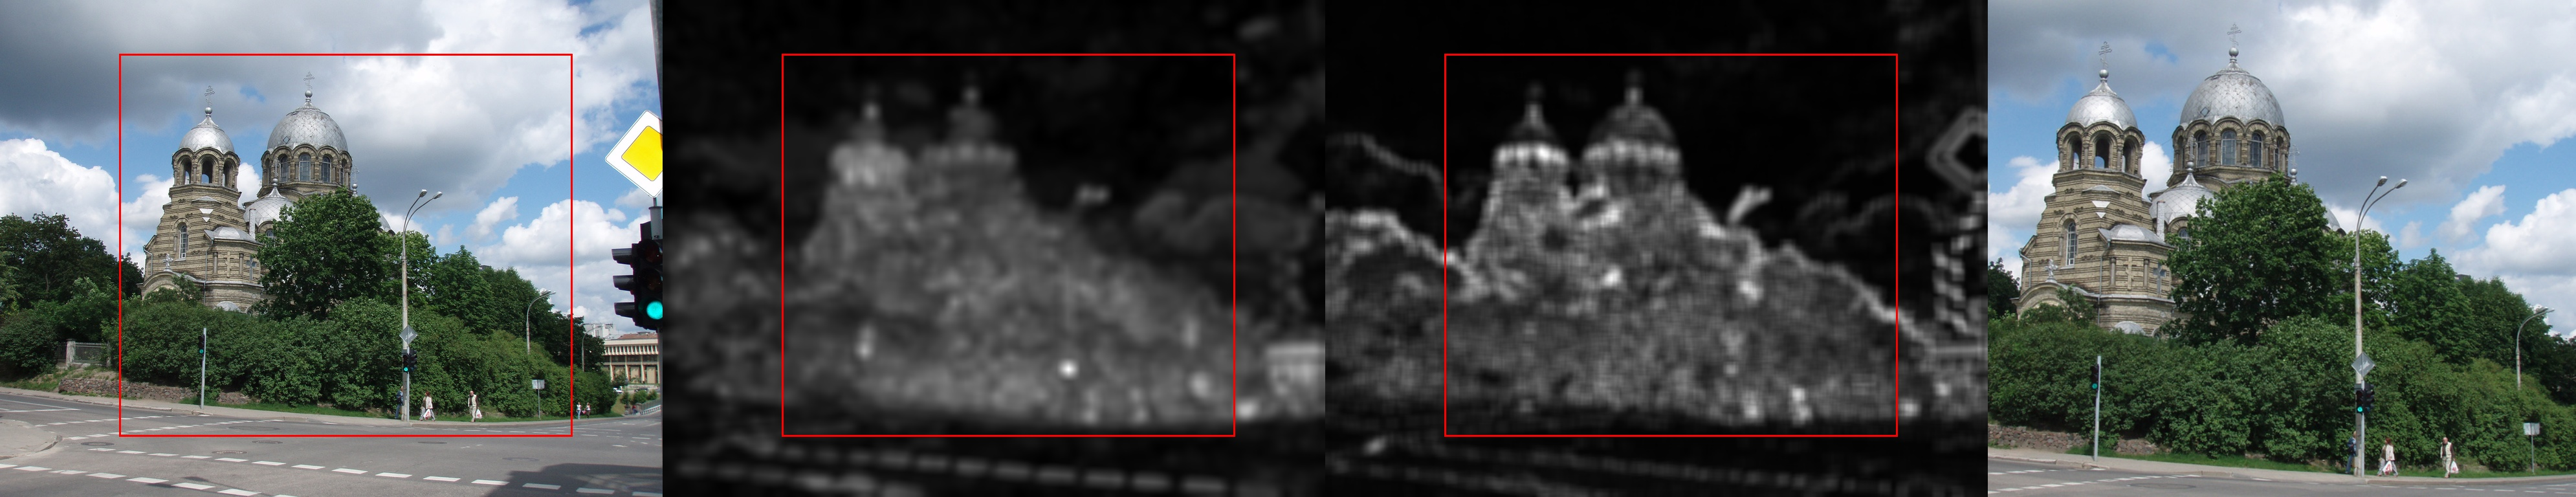
\includegraphics[width=0.9\columnwidth]{../figures/Chen_crops/simple_boundary/1022974255_Large.jpg}
\vskip3pt
\centering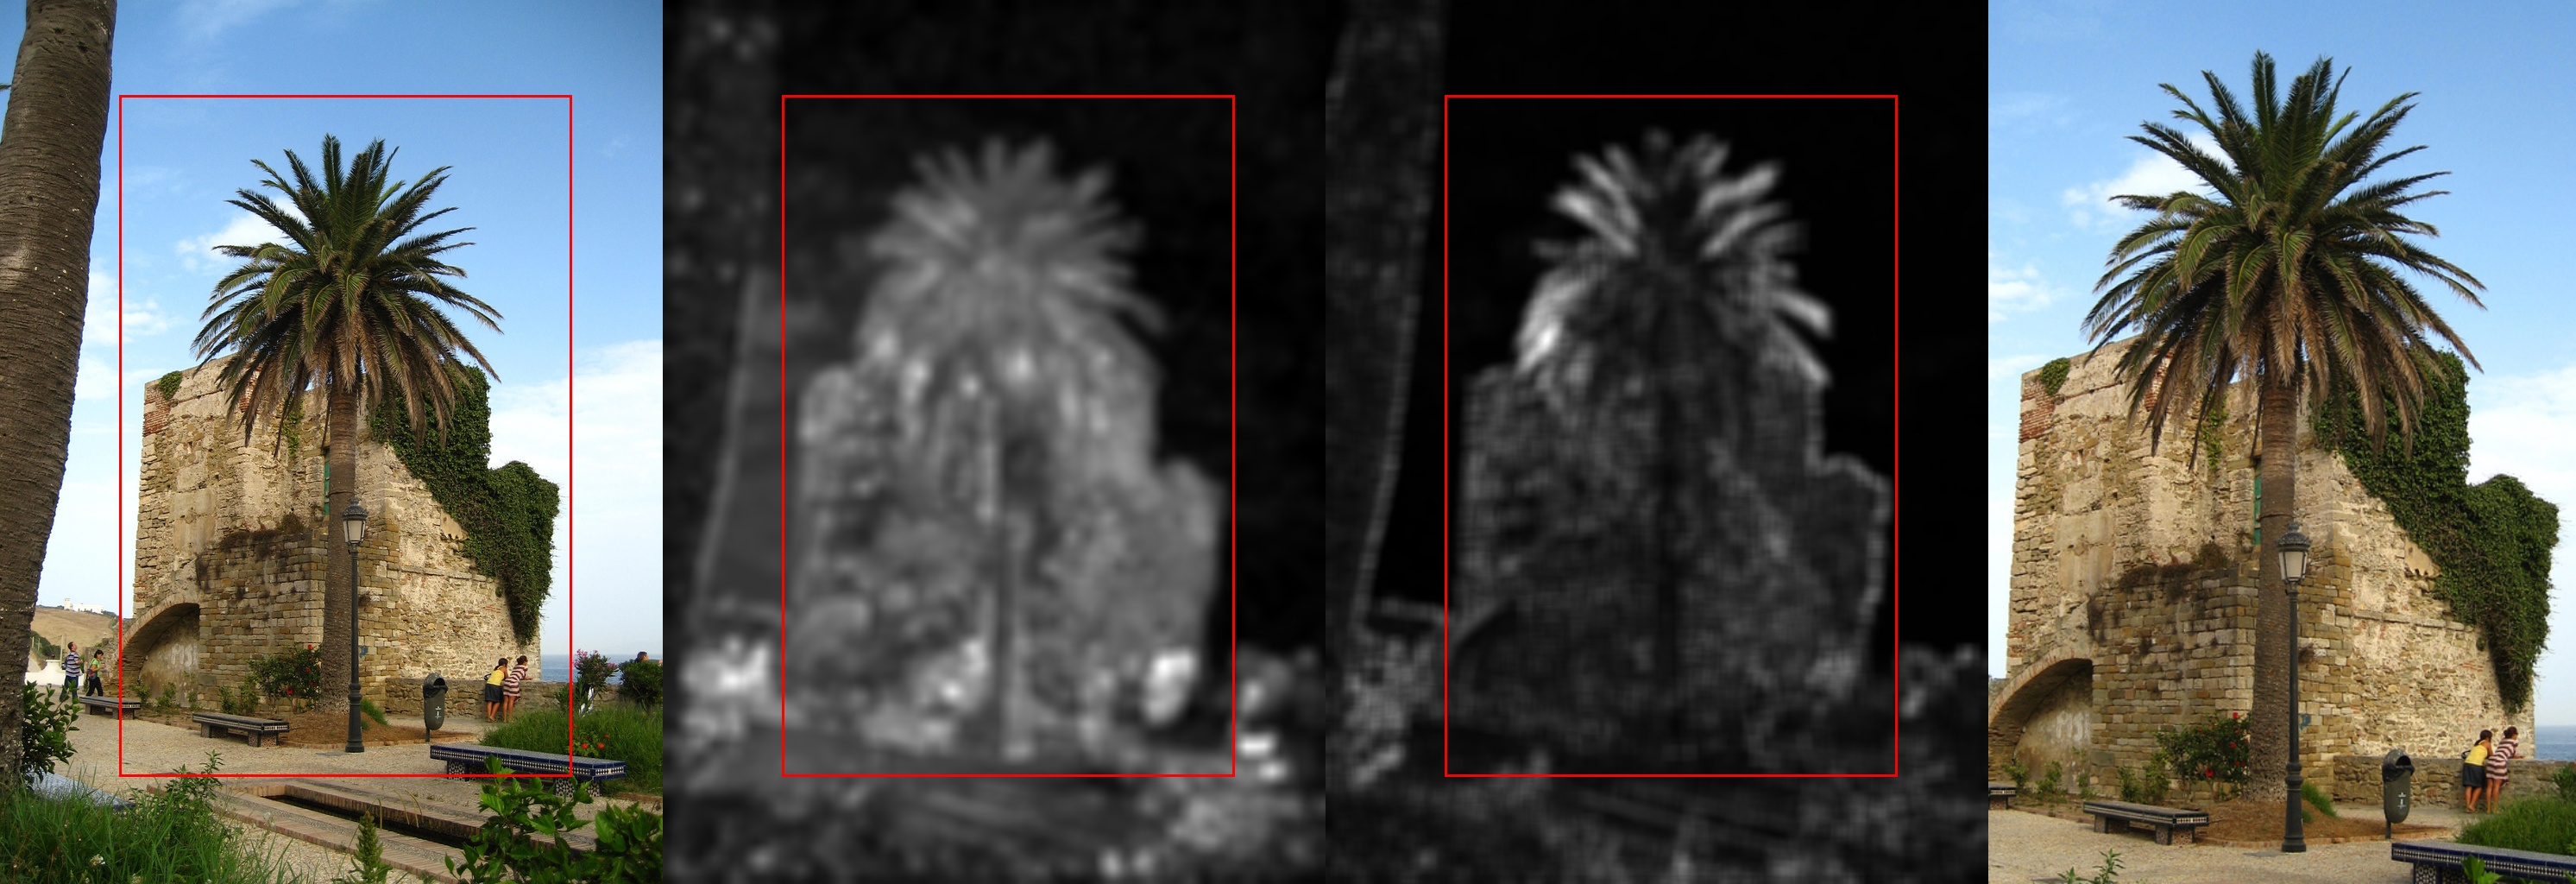
\includegraphics[width=0.9\columnwidth]{../figures/Chen_crops/simple_boundary/1192872104_Large.jpg}
\vskip3pt
\centering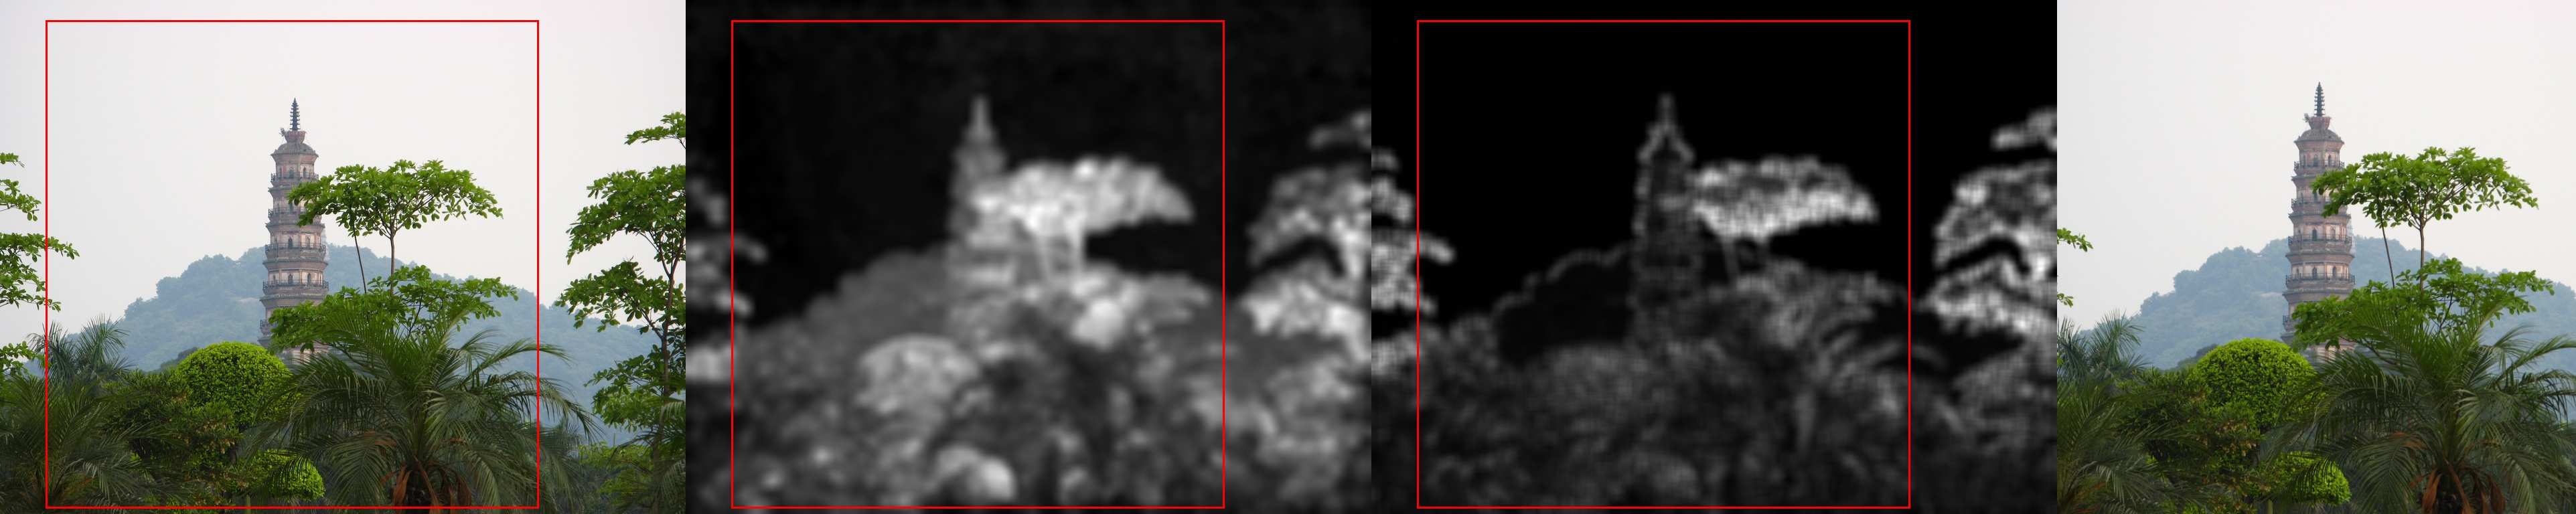
\includegraphics[width=0.9\columnwidth]{../figures/Chen_crops/simple_boundary/504325680_Large.jpg}
\vskip3pt
\centering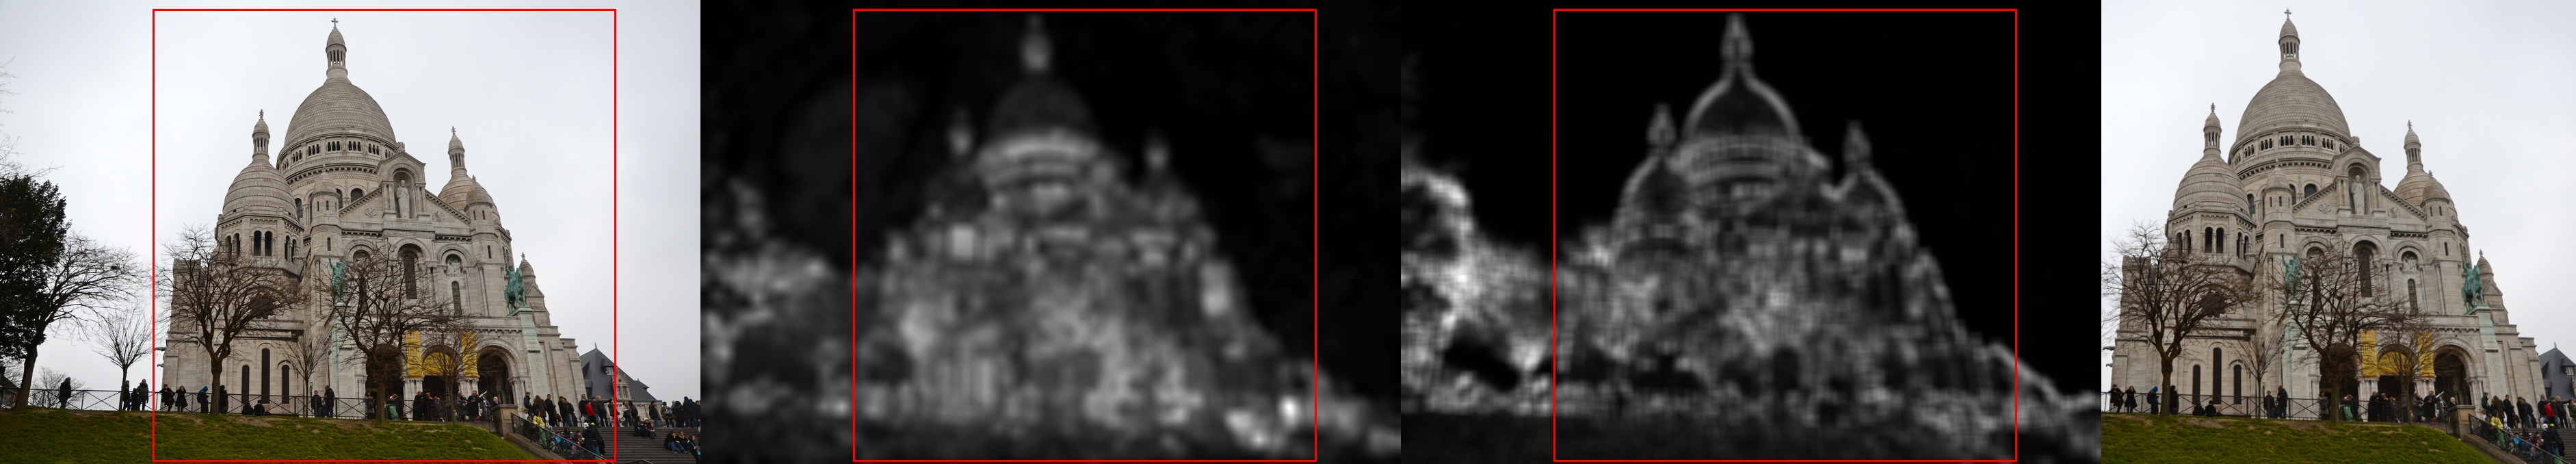
\includegraphics[width=0.9\columnwidth]{../figures/Chen_crops/simple_boundary/6853433974_Large.jpg}
\vskip3pt
\small{(From left to right: original image, saliency map, gradient map, final cropped image)}
\caption{Crops with good boundary simplicity.\label{fig:cropped_simplicity}}
\end{figure}

The automatic cropper does have its pitfalls however.
The most common error occurs when the final crop cuts through distinct
foreground objects.
This is shown well in figure \ref{fig:cropped_cutobject}.
It can be seen especially well for the case of the first image that the fault
may lie in the saliency map implementation used.
Other background colours and patterns are deemed more salient at times making
it more challenging for the algorithm to retain relevant but "not salient"
regions.

\begin{figure}
\centering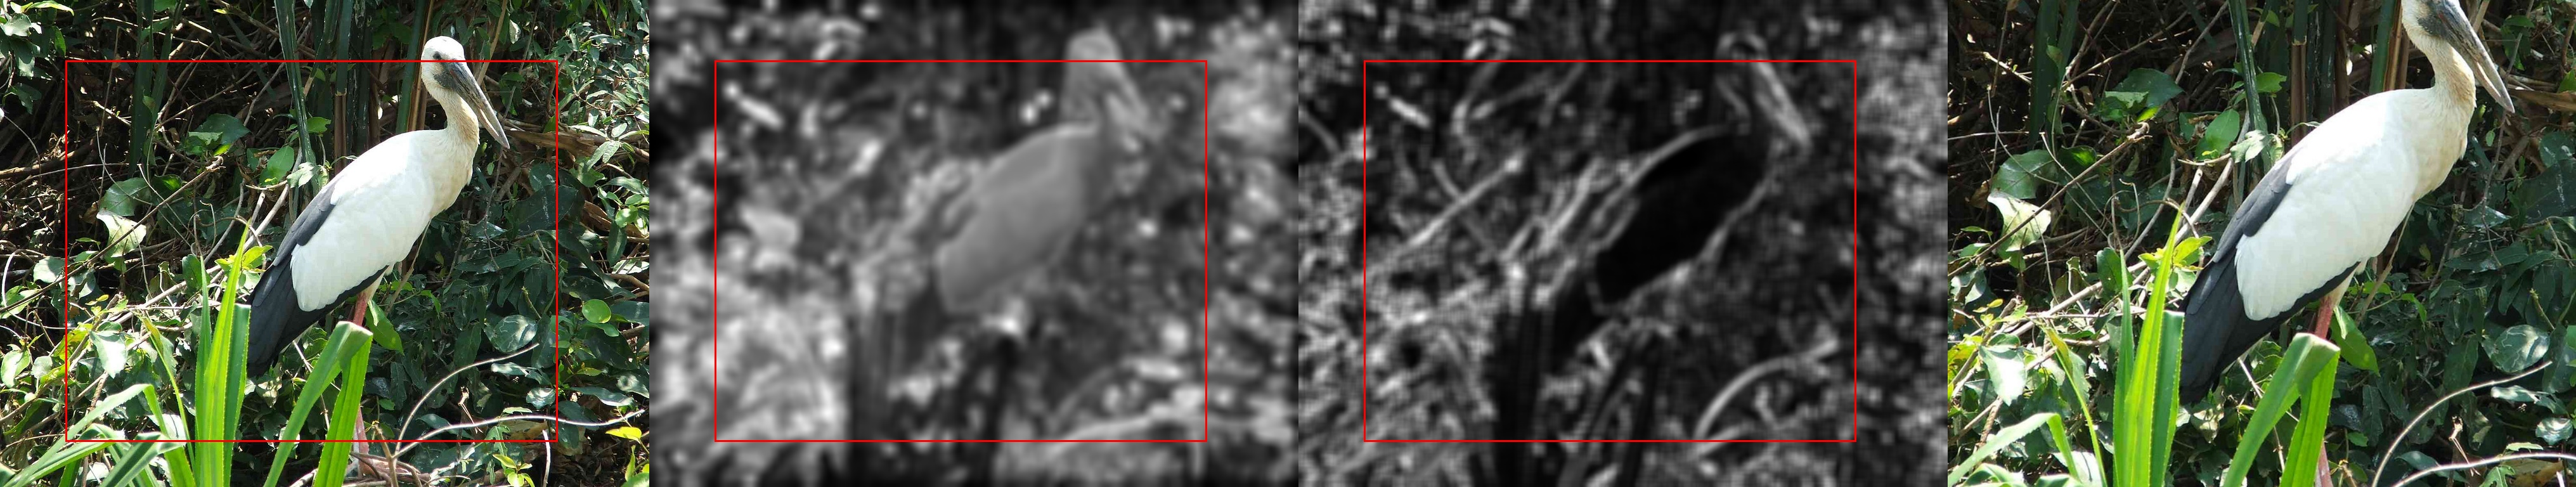
\includegraphics[width=0.9\columnwidth]{../figures/Chen_crops/cut_object/118697470_Large.jpg}
\vskip3pt
\centering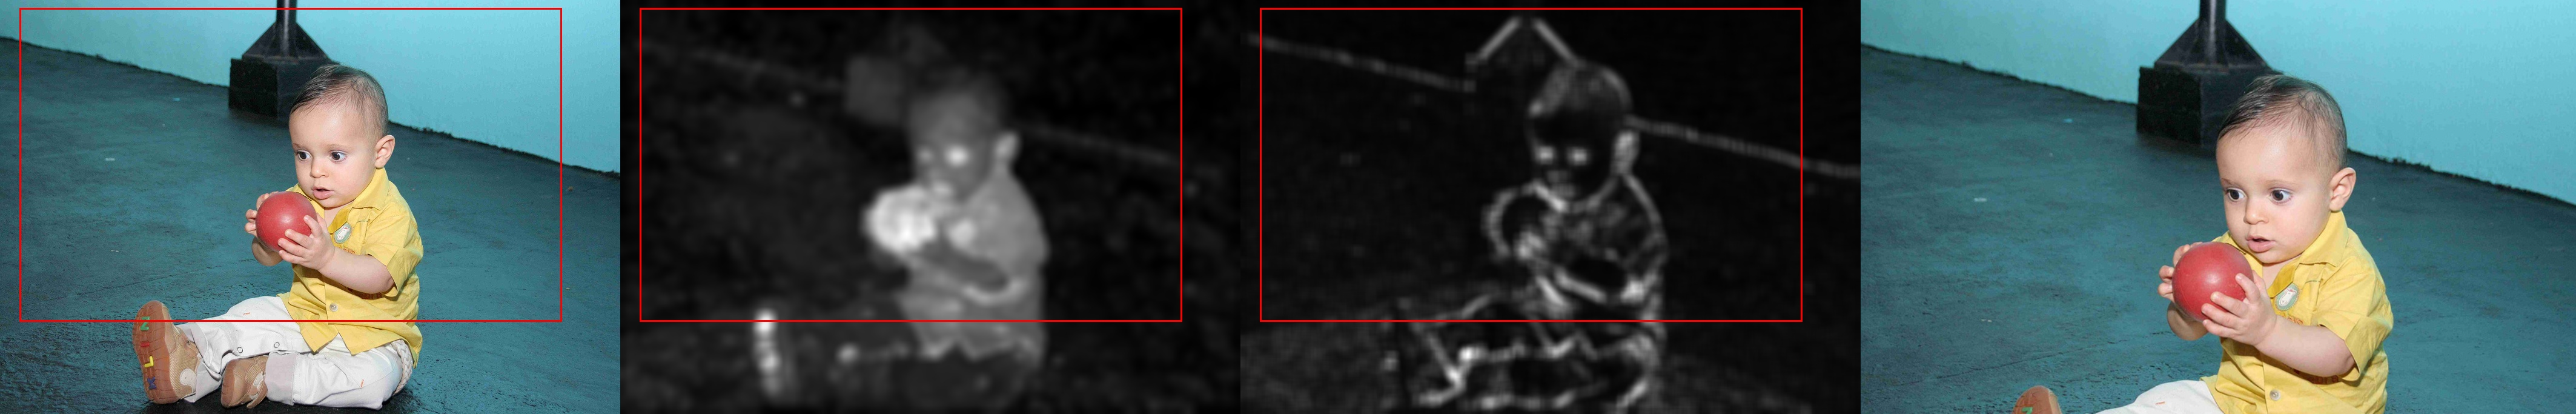
\includegraphics[width=0.9\columnwidth]{../figures/Chen_crops/cut_object/1347846010_Large.jpg}
\vskip3pt
\centering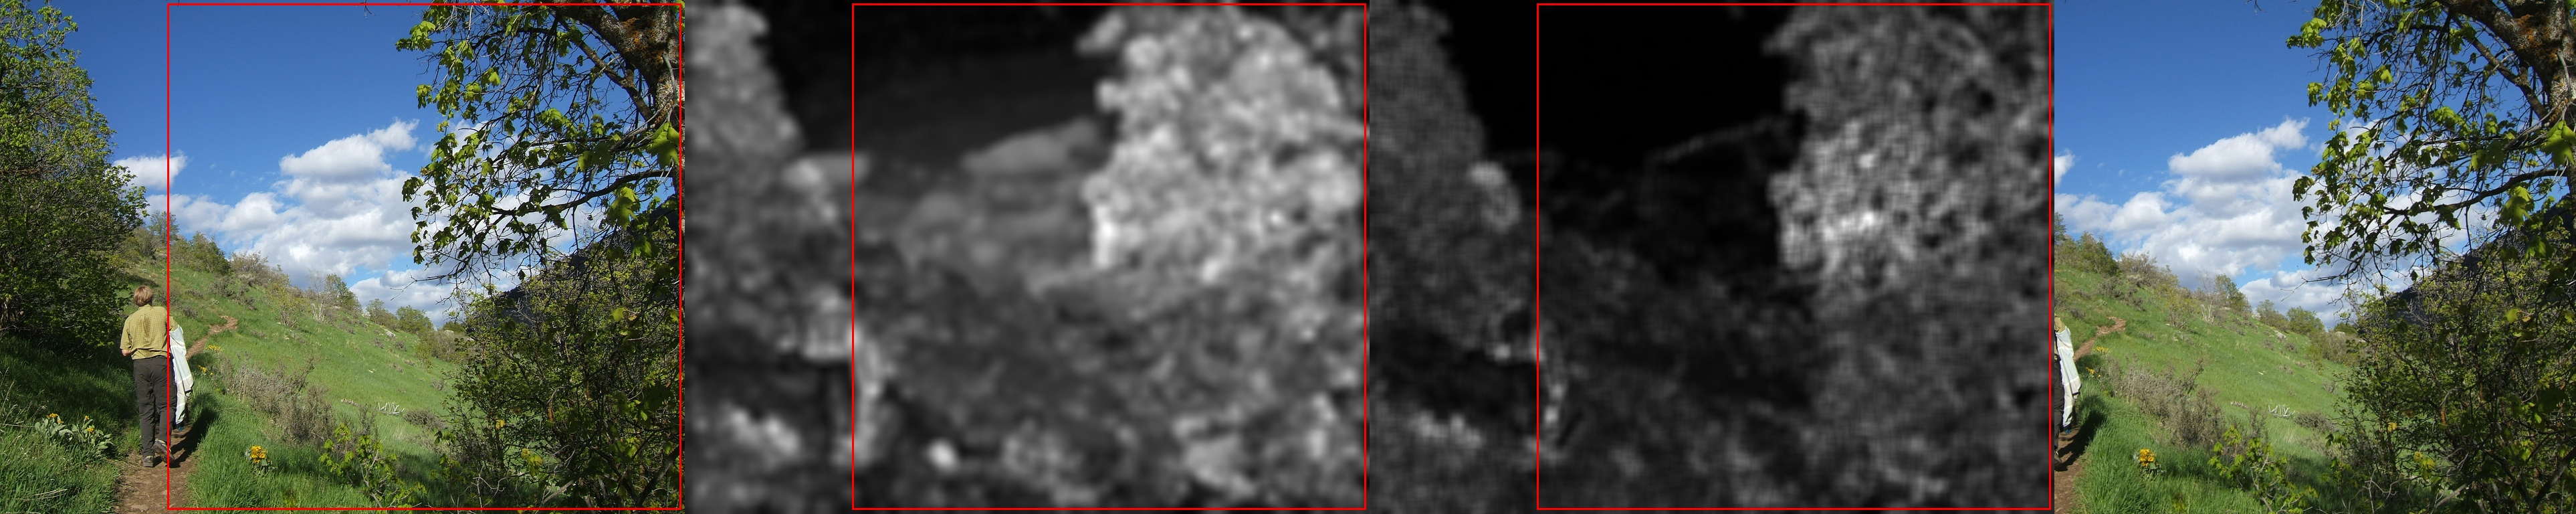
\includegraphics[width=0.9\columnwidth]{../figures/Chen_crops/cut_object/490466578_Large.jpg}
\vskip3pt
\centering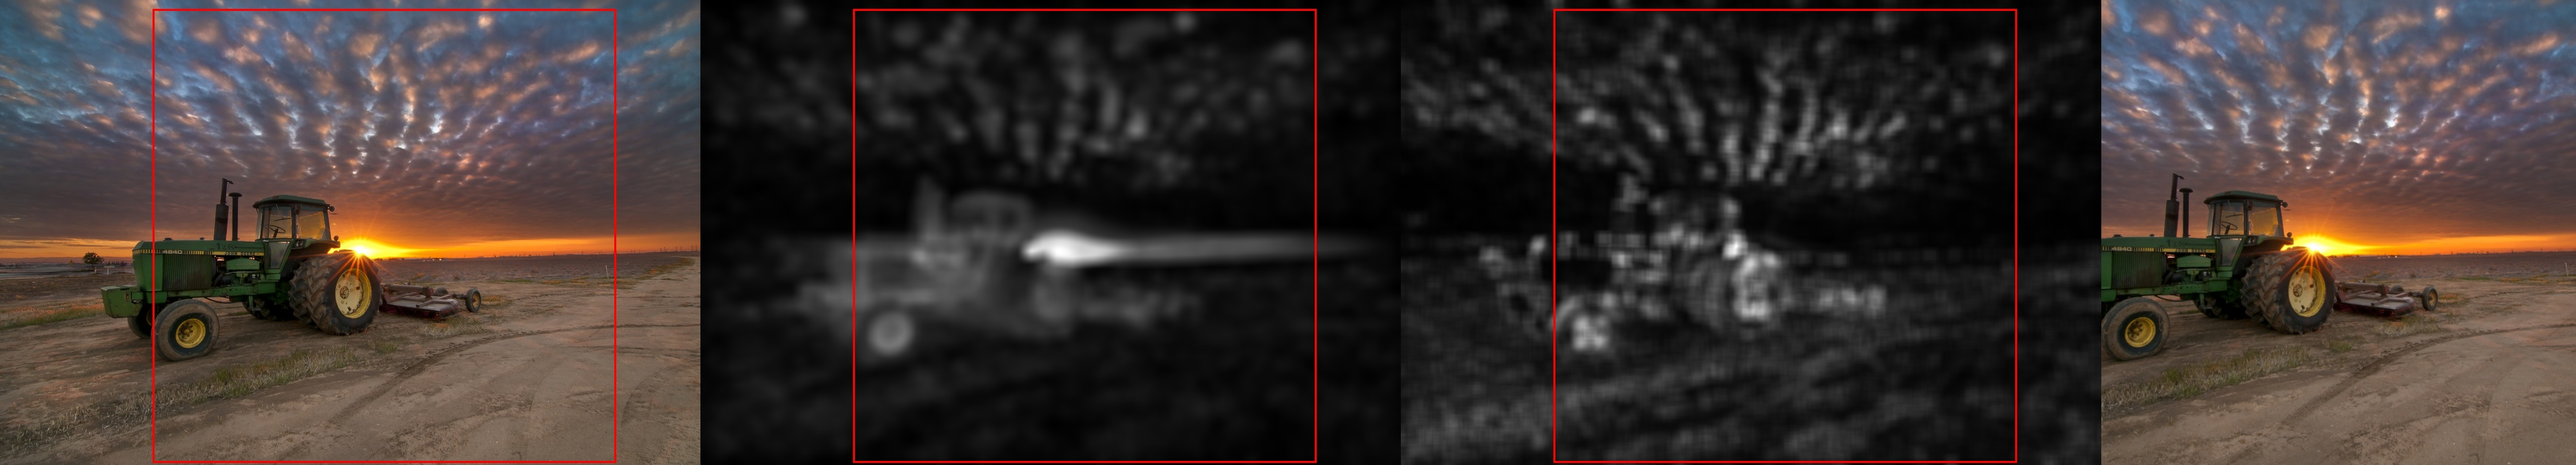
\includegraphics[width=0.9\columnwidth]{../figures/Chen_crops/cut_object/6853040778_Large.jpg}
\vskip3pt
\small{(From left to right: original image, saliency map, gradient map, final cropped image)}
\caption{Unideal crops which cut through objects.\label{fig:cropped_cutobject}}
\end{figure}

Another example where the saliency map implementation may cause issues is when
reflections occur in an input image.
Figure \ref{fig:cropped_reflection} shows an example with a flock of flamingoes
and their reflection.
Both the flock and their reflection is considered salient and thus the final
crop is not composed as well as the initial image.
This could be a cause for confusion for human croppers as well however,
especially when a reflection could be considered artistic and thus should be
well focused.

\begin{figure}
\centering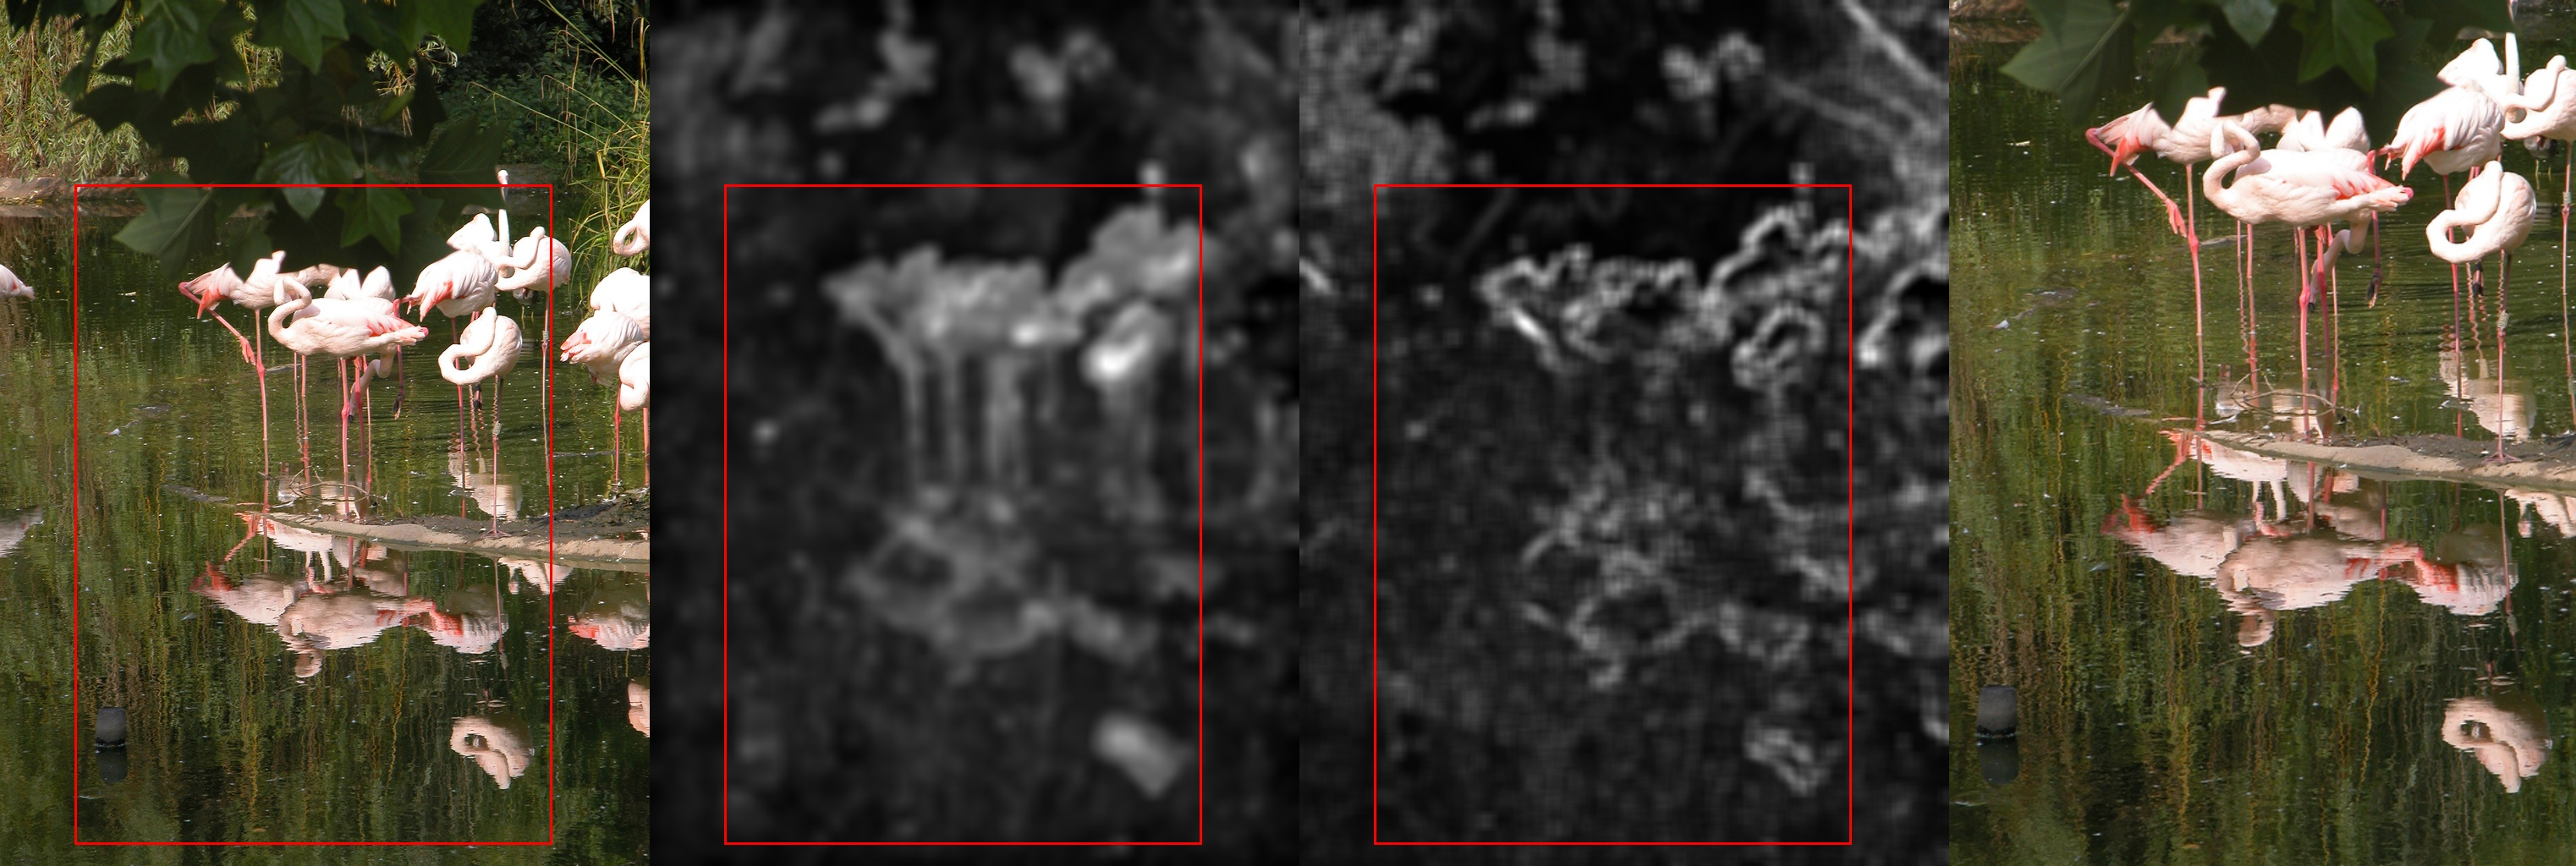
\includegraphics[width=0.9\columnwidth]{../figures/Chen_crops/reflections/46152273_Large.jpg}
\vskip3pt
\small{(From left to right: original image, saliency map, gradient map, final cropped image)}
\caption{Unideal crop due to reflections.\label{fig:cropped_reflection}}
\end{figure}

Overall, the automatic cropping algorithm works very well.
Any mistakes could be improved in the future with better saliency map
implementations.


